\documentclass{article}
\usepackage{mathtools}
\usepackage{graphicx}
\usepackage{titling}  % For custom title page
\usepackage{circuitikz}
\usepackage{matlab-prettifier}
\usepackage{amsmath}
\usepackage{amssymb}
\usepackage{booktabs,tabu}
\usepackage[section]{placeins}
\DeclarePairedDelimiter\ceil{\lceil}{\rceil}
\DeclarePairedDelimiter\floor{\lfloor}{\rfloor}

\title{Experiment 5: Power Spectrum Estimation}
\author{Samyak Sheersh}
\date{2 October 2024}
\newcommand{\subtitle}[1]{%
  \posttitle{%
    \par\end{center}
    \begin{center}\large#1\end{center}
    \vskip0.5em}%
}

\begin{document}

% Custom title page
\begin{titlepage}
    \centering
    
\includegraphics[width=0.2\textwidth]{KGP_logo.png}\par\vspace{1cm}
    {\scshape\LARGE Department of Electronics and Electrical Communication Engineering, IIT Kharagpur\par}
    \vspace{1cm}
    {\huge\bfseries Experiment 5: Power Spectrum Estimation \par}
    \vspace{1.5cm}
    {\Large\itshape Samyak Sheersh, Anubhav Mitra\par}
    \vfill
    % Identifying information at the bottom
    {\large Roll Numbers: 22EC30045, 22EC30007\par}
    {\large Group Number: 24\par}
    \vfill
    {\large 22 October 2024\par}
\end{titlepage}

\section{Objectives}
\begin{enumerate}
  \item To generate a random signal $x[n]$ with a known Power Spectral Density(PSD) by passing it through a filter $H(z)$.
  \item We then use two techniques to find out the PSD, and in the process measure their accuracy and other properties. In particular, we will use:

    \begin{enumerate}
      \item The Welch Non-parametric method: Averaging a modified periodogram.
      \item The Yule-Walker AR model: A parametric method of power spectrum estimation. 
    \end{enumerate}
\end{enumerate}
\section{Procedure}
\subsection{Task 1: Generating the signal}
We generate a random normally distributed signal $r_w[n]\sim N(\mu=0,\sigma^2)$ and pass it through a digital filter $H(z)$ where:
\begin{equation}
    H(z)=\frac{1}{(1-0.9z^{-1})(1-0.9jz^{-1})(1+0.9jz^{-1})}
\end{equation}

to get $x[n]$. Thus ensuring that the Power spectral density of $x[n]$ is
\begin{equation}
  P_{xx}(f)=|H(e^{j2\pi f})|^2 \cdot \sigma^2
\end{equation}

\subsection{Task 2: The Welch Non-Parametric method}
We know that the PSD of $x[n]$ is:
\begin{equation}
  P_{xx}(f)=\lim_{N\rightarrow \infty} \frac{1}{2N+1} E\Big\{\Big|\sum_{n=-N}^{N} x[n] e^{-j2\pi fn}\Big|^2\Big\}
\end{equation}

for a periodogram, we make a the sum over a finite $0$ to $N-1$($N$ samples from $t=0$), and drop the estimate sign, to get the expression:
\begin{equation}
    \hat{P}_{xx}(f)=\frac{1}{N}\Big|\sum_{n=0}^{N-1}x[n] e^{-j2\pi fn}\Big|^2
\end{equation}
where the $\hat{P}$ is used to denote that this is an estimator for the true $P$. In this case, this is the Naive estimator $\hat{X}=X_i$


It can be shown that this is an asymptotically unbiased estimator, but the variance doesn't decay to $0$ as $N\rightarrow \infty$. However, to overcome this (i.e. to reduce the variance), we can use the result from Central Limit Theorem that the variance of the sample mean reduces by $1/n$ as the number of samples(in this case, the number of periodograms we generate) $n$ increases. So we generate a lot of periodograms from different parts of the signal and take their mean to come to an estimate. 

The Welch method also introduces a windowing function and overlapping segments:
\begin{enumerate}
  \item We divide $x[n]$ into $L$(typically $L=8$) overlapping blocks of length $M$ and an overlap of $D$ between consecutive blocks.Such that for the $i^{th}$ block:
    \begin{equation}
      x_i[n]=x[n+i(M-D)]
    \end{equation}
    where $0\leq n< M$ and $0\leq i< L$.

    This also gives us a way to calculate $M$ in terms of the $N,L$ and $D$ as:
    \begin{equation}
      x[M-1+(L-1)(M-D)]=x[N-1]
    \end{equation}
    \begin{equation}
      \Rightarrow M=\Bigg\lceil\frac{N+(L-1)D}{L}\Bigg\rceil
    \end{equation}
    Since we know D as a fraction of M($D=dM$, where d is the percentage of overlap), we can write:
    \begin{equation}
      \Rightarrow M=\Bigg\lceil\frac{N}{L-(L-1)d}\Bigg\rceil
    \end{equation}
  \item We then obtain the estimated PSD of the $i^{th}$ block as:
    \begin{equation}
      \hat{P}_{xx}^{(i)}(f)= \frac{1}{MU}\Bigg|\sum_{n=0}^{M-1}x_i(n)w(n) e^{-j2\pi fn}\Bigg|^2; 0\leq i< L
    \end{equation}
    where $w(n)$ is a (usually Hamming) Window function of length $M$, and $U$ is the normalisation factor(the energy of the window function):
    \begin{equation}
        U=\frac{1}{M}\sum_{n=0}^{M-1}w(n)^2
    \end{equation}
  \item We then obtain the Welch spectrum estimate by the average of these modified periodograms:
    \begin{equation}
      P^{W}_{xx}(f)=\frac{1}{L}\sum_{i=0}^{L-1}\hat{P}_{xx}^{(i)}(f)
    \end{equation}
\end{enumerate}

\subsection{Task 3: The Yule-Walker AR Method}
We can do a much better job of getting an estimated PSD if we know how the signal was generated(i.e. a prior knowledge regarding the source of data generation). We also don't require any Windowing in this method since all samples would be assumed to come from the same process. This is particularly useful for generating PSDs of signals of which we only have a short segment, since we'll only have to converge to a few parameters. This is the approach behind Yule-Walker AR Method.

One of the simplest models is an autoregressive model of $p^{th}$ order. The equation looks like:
\begin{equation}
  y[n]=\phi_1 y[n-1]+\phi_2 y[n-2]+\ldots+\phi_p y[n-p]+\epsilon[n]
\end{equation}
where $\epsilon[n]$ is random noise. If we treat this as a system with the random noise as an input into it. The transfer function is:
\begin{align}
  Y(z)(1-\phi_1 z^{-1}-\phi_2 z^{-2}-\ldots-\phi_p z^{-p})=X(z)\\
  \Rightarrow H(z)=\frac{Y(z)}{X(z)}=\frac{1}{(1-\phi_1 z^{-1}-\phi_2 z^{-2}-\ldots-\phi_p z^{-p})}\\
  \Rightarrow H(z)=\frac{1}{1-\sum_{n=1}^{p}\phi_n z^{-n}}=\frac{1}{1+\sum_{n=1}^{p}a_n z^{-n}}
\end{align}
where $a_i=-\phi_i$, $X(z)$ is the input signal and $Y(z)$ is the output signal. To obtain the PSD of our sequence $x[n]$, we can apply the Yule-Walker AR method to estimate the $H(z)$ that generates $x[n]$ and then plot $\sigma^2 |H(e^{j2\pi f})|^2$


\begin{enumerate}
  \item We calculate the autocorrelation function(+ve lags only) as:
    \begin{equation}
      R_{xx}[n]=\frac{1}{N}\sum_{m=0}^{N-n-1}x[m]x[m+n]; 0\leq n<N
    \end{equation}
  \item We then solve the Yule-Walker AR model to get $a_i$:
    \begin{equation}
    \begin{pmatrix}
      R_{xx}(0) & R_{xx}(1)  & \ldots & R_{xx}(p-1)\\
      R_{xx}(1) & R_{xx}(0)  & \ldots & R_{xx}(p-2)\\
      \vdots & \vdots & \ddots & \vdots\\
      R_{xx}(p-1) & R_{xx}(p-2) & \ldots & R_{xx}(0)\\
    \end{pmatrix}
    \begin{pmatrix}
      a_1\\
      a_2\\
      \vdots\\
      a_p
    \end{pmatrix}
    =-
    \begin{pmatrix}
      R_{xx}(1)\\
      R_{xx}(2)\\
      \vdots\\
      R_{xx}(p)
    \end{pmatrix}
    \end{equation}
    where $A_{ij}=R_{xx}(|i-j|)$
  \item We then estimate the variance of $x[n]$ as:
    \begin{equation}
      \sigma^2_{rp}=R_{xx}[0]+\sum_{i=1}^{p}a_i R_{xx}[i]
    \end{equation}
  \item We then construct the transfer function $\hat{H}(z)$ as:
    \begin{equation}
      \hat{H}(z)=\frac{1}{1+\sum_{i=1}^{p}a_i z^{-i}}
    \end{equation}
    and thus the estimated PSD as such:
    \begin{equation}
      P^{YW}_{xx}(f)=\sigma^2_{rp}|\hat{H}(e^{j2\pi f})|^2=\frac{\sigma^2_{rp}}{|1+\sum_{k=1}^{p}a_k e^{-j2\pi fk}|^2}
    \end{equation}
\end{enumerate}
\clearpage
\section{Results}
\subsection{Task 1}
\begin{figure}[!ht]
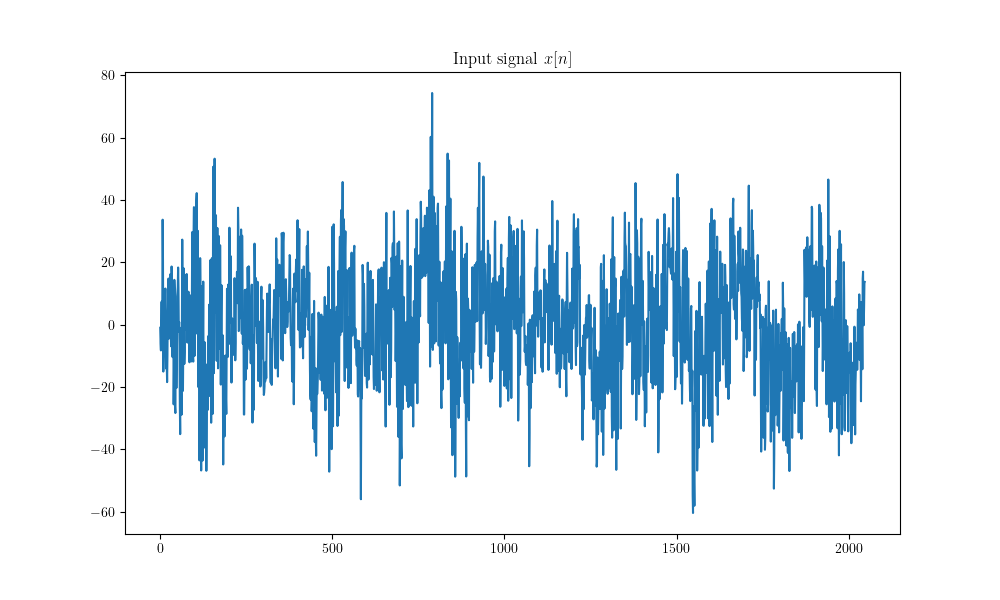
\includegraphics[width=\textwidth]{x_n.png}
\caption{Signal $x[n]$ with $N=2048$}
\label{fig:x_n}
\end{figure}
\begin{figure}[!ht]
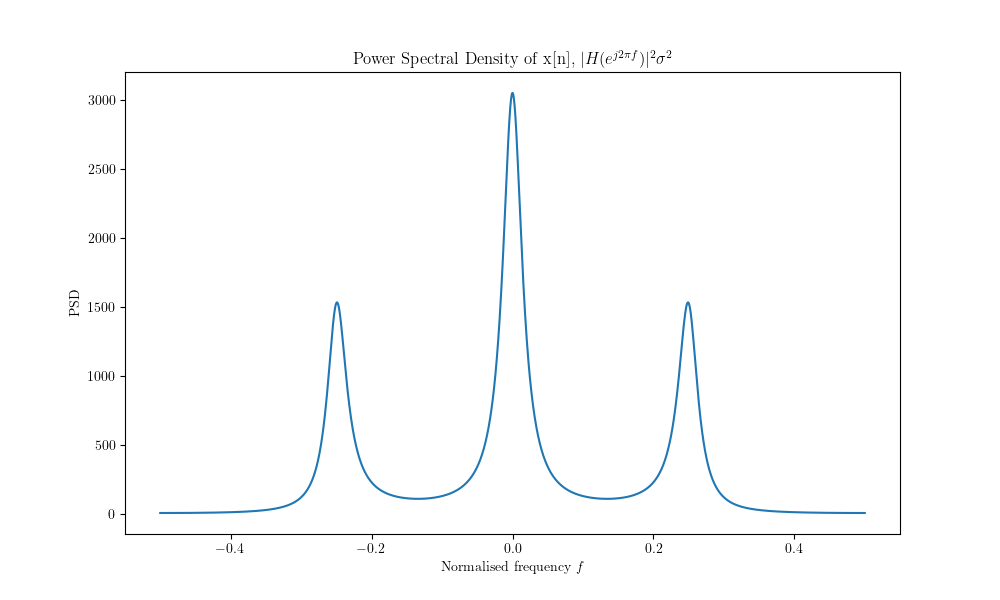
\includegraphics[width=\textwidth]{PSD_t.png}
\caption{Theoretical PSD of $x[n]$, $N=2048$}
\label{fig:psdt}
\end{figure}
\clearpage
\subsection{Task 2}
\begin{figure}[!ht]
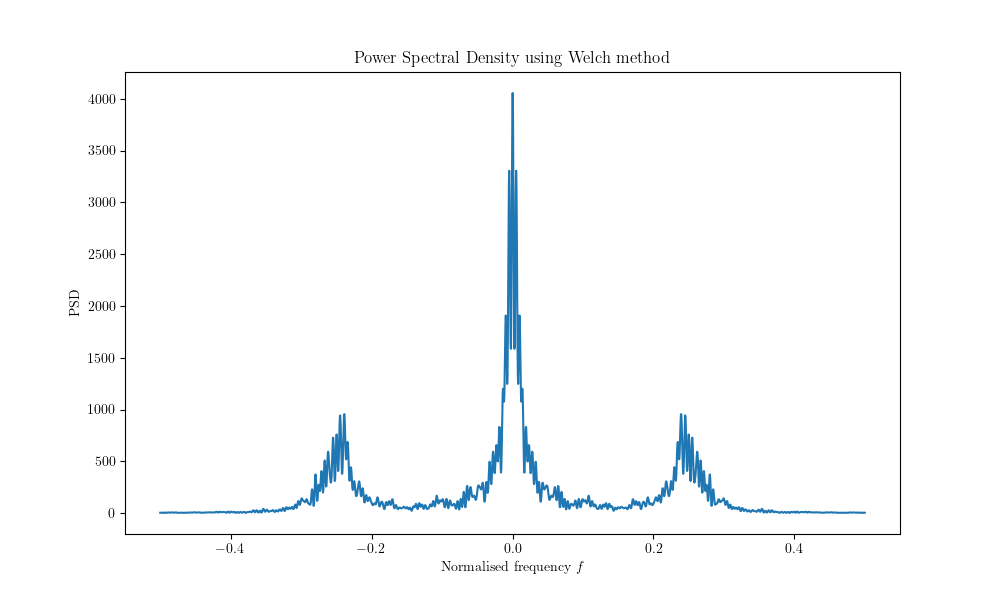
\includegraphics[width=\textwidth]{PSD_Welch_0.png}
\caption{PSD using Welch method with $D=0$}
\label{fig:psdw0}
\end{figure}

\begin{figure}[!ht]
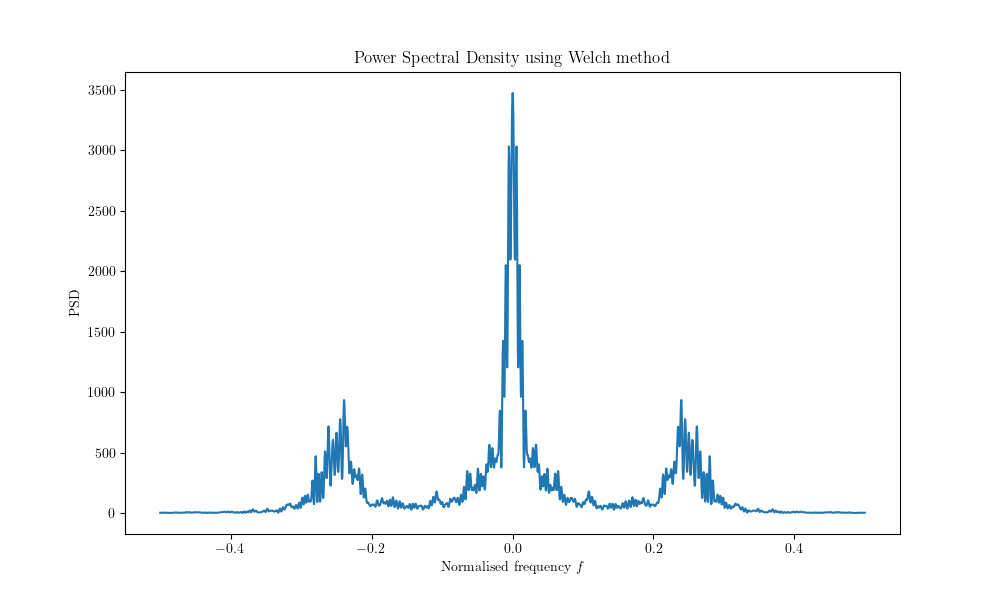
\includegraphics[width=\textwidth]{PSD_Welch_0.1.png}
\caption{PSD using Welch method with $10\%$ overlap}
\label{fig:psdw0.1}
\end{figure}

\begin{figure}[!ht]
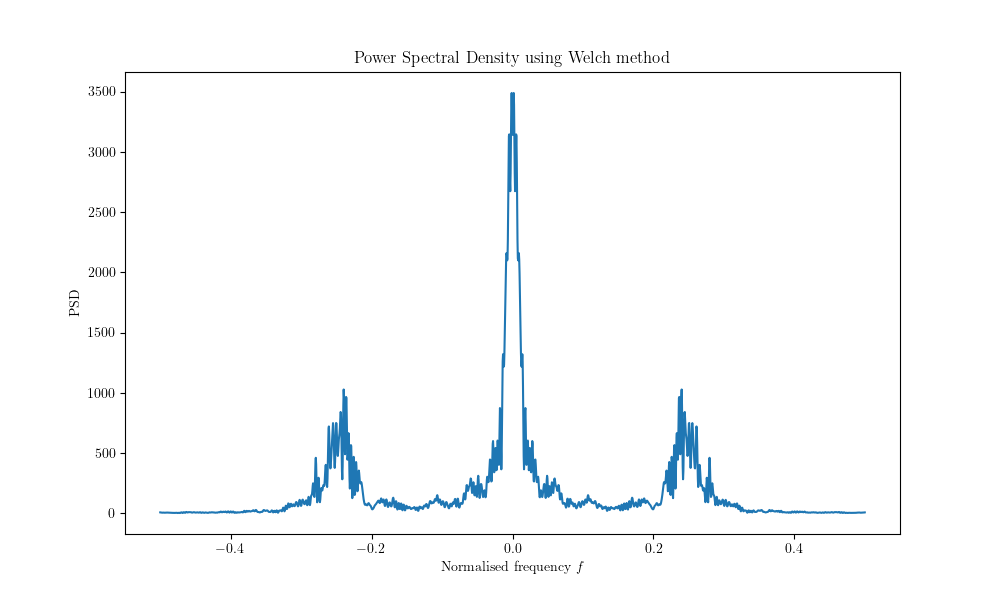
\includegraphics[width=\textwidth]{PSD_Welch_0.25.png}
\caption{PSD using Welch method with $25\%$ overlap}
\label{fig:psdw0.25}
\end{figure}

\begin{figure}[!ht]
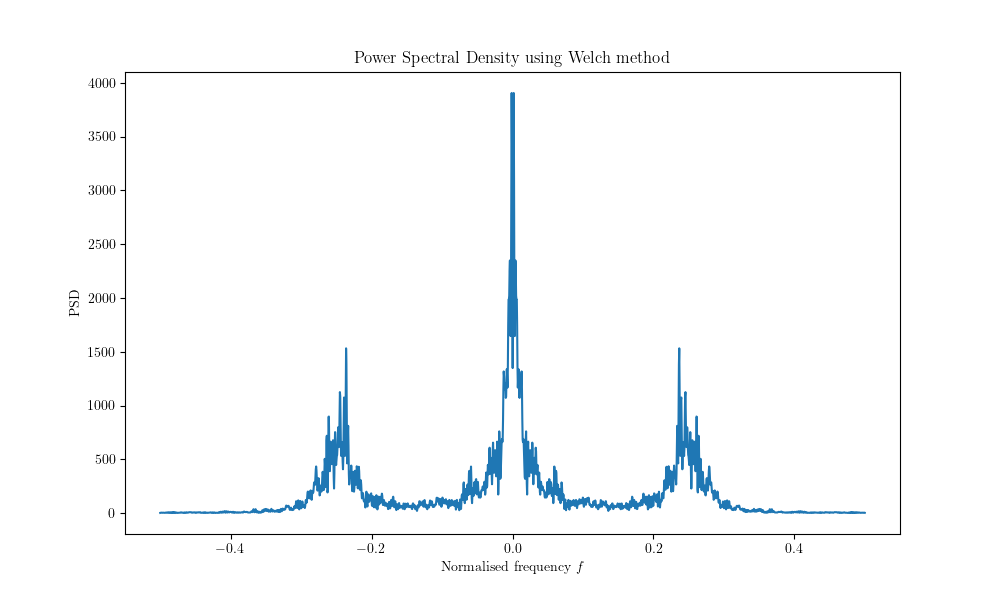
\includegraphics[width=\textwidth]{PSD_Welch_0.5.png}
\caption{PSD using Welch method with $50\%$ overlap}
\label{fig:psdw0.5}
\end{figure}
\clearpage
\subsection{Task 3}
\begin{figure}[!ht]
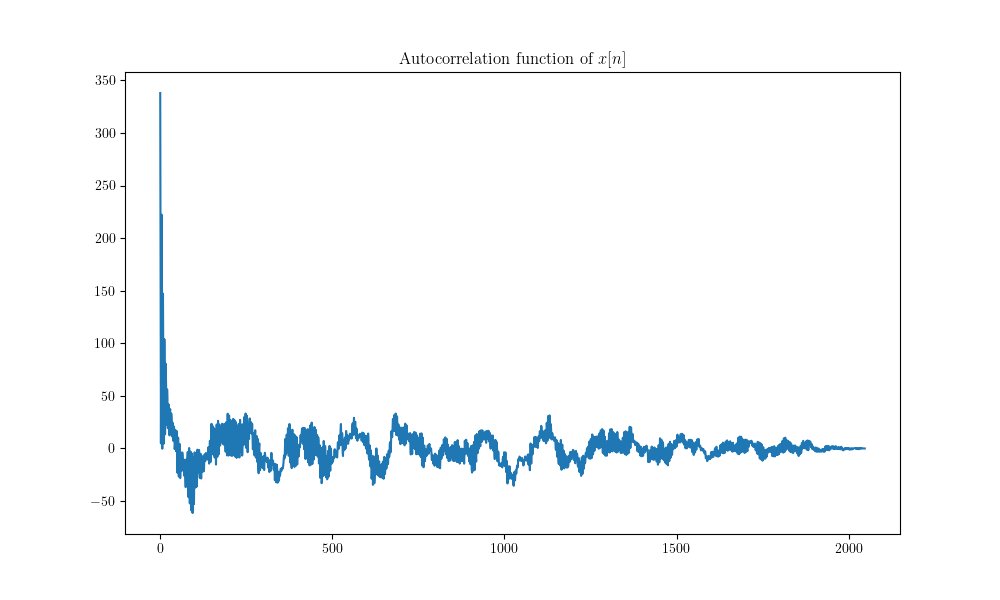
\includegraphics[width=\textwidth]{ACF.png}
\caption{Autocorrelation function of $x[n]$}
\label{fig:acf}
\end{figure}

\begin{figure}[!ht]
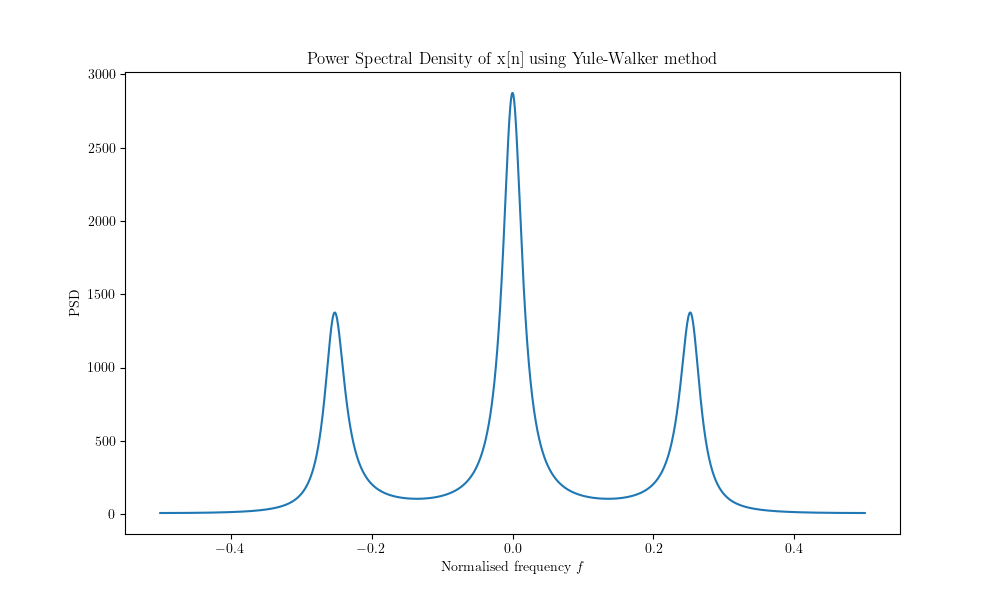
\includegraphics[width=\textwidth]{PSD_YW_3.png}
\caption{PSD using Yule-Walker method with $p=3^{th}$ AR model}
\label{fig:psdyw3}
\end{figure}

\begin{figure}[!ht]
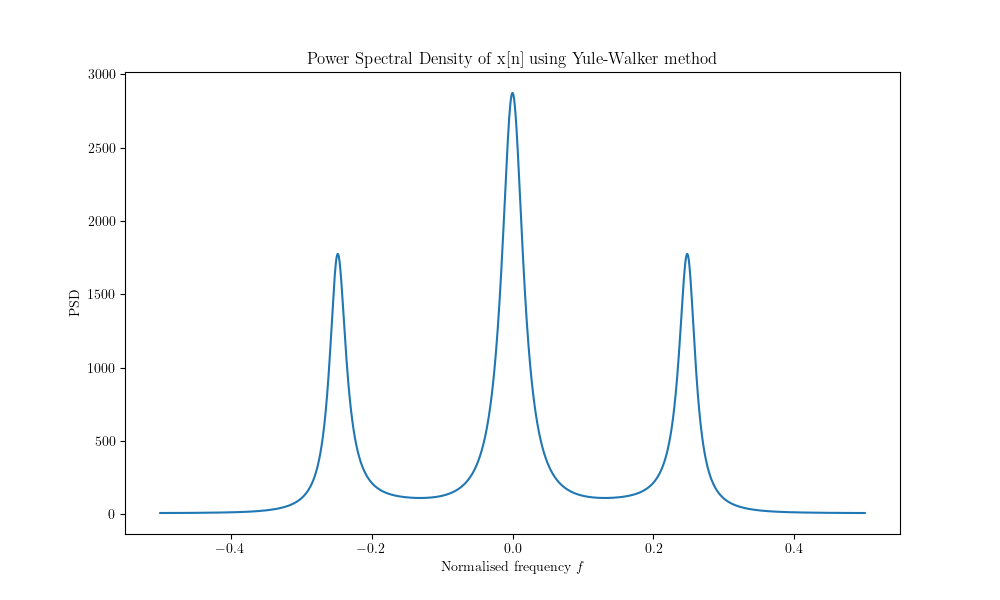
\includegraphics[width=\textwidth]{PSD_YW_10.png}
\caption{PSD using Yule-Walker method with $p=10^{th}$ AR model}
\label{fig:psdyw10}
\end{figure}

\begin{figure}[!ht]
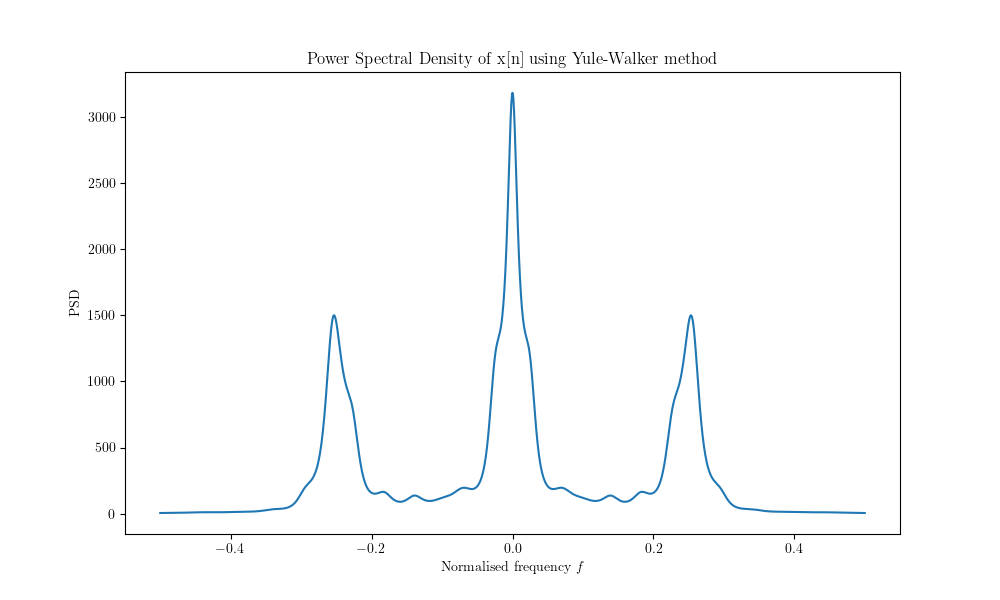
\includegraphics[width=\textwidth]{PSD_YW_30.png}
\caption{PSD using Yule-Walker method with $p=30^{th}$ AR model}
\label{fig:psdyw30}
\end{figure}

\begin{figure}[!ht]
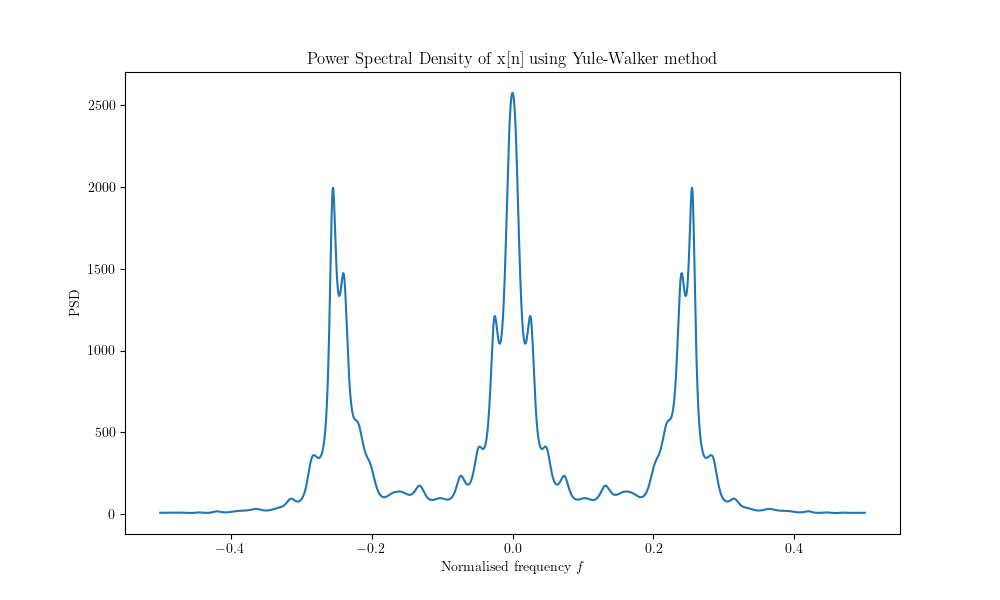
\includegraphics[width=\textwidth]{PSD_YW_50.png}
\caption{PSD using Yule-Walker method with $p=50^{th}$ AR model}
\label{fig:psdyw50}
\end{figure}

\begin{figure}[!ht]
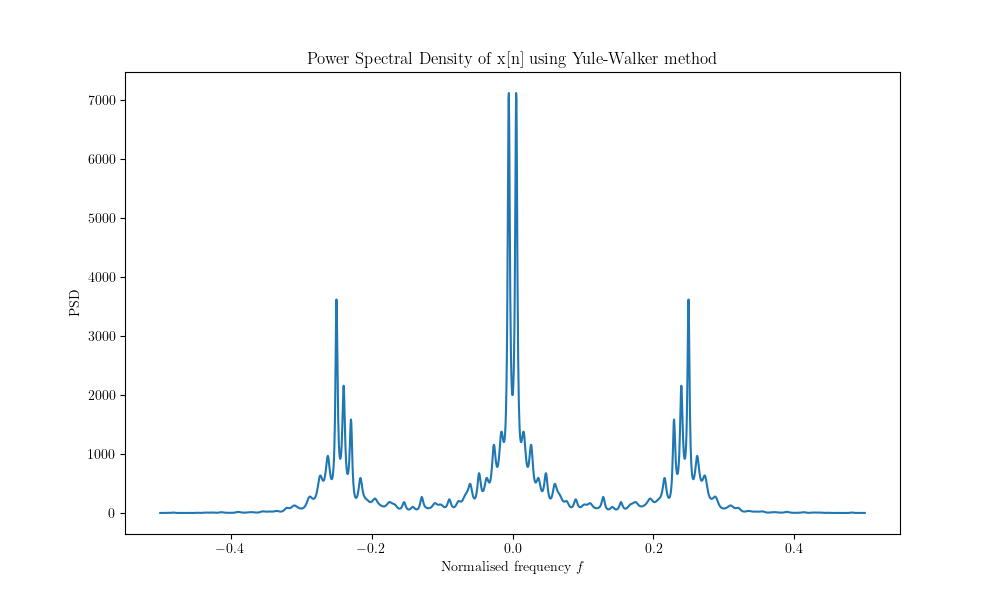
\includegraphics[width=\textwidth]{PSD_YW_100.png}
\caption{PSD using Yule-Walker method with $p=100^{th}$ AR model}
\label{fig:psdyw100}
\end{figure}
\section{Discussion: Samyak Sheersh}
\begin{enumerate}
  \item We saw for the Welch Method, that as the overlap $D$ increased, the estimate of the PSD converged up until 50\% overlap(see Figures \ref{fig:psdw0}, \ref{fig:psdw0.1}, \ref{fig:psdw0.25}, and \ref{fig:psdw0.5}). After that the accuracy actually started worsening (the lines became thicker and more uncertain), probably because some values in the middle got a much stronger influence on the final PSD due to being considered multiple times.
  \item The PSD using Welch method was also more noisy than the one using Yule-Walker models. This was expected since the Welch method has to converge to a whole distribution which has a lot more variables and thus a lot more uncertainity, while the Yule-Walker generates a totally new mdoel from the few parameter it infers.
  \item The autocorrelation function(see Figure \ref{fig:acf}) quickly decayed to $0$ for increasing $n$, as expected, since the signal is not periodic or with a coherent structure 
  \item As we had put in a random signal through a known PSD, we had known that is was an AR(3) model(the transfer function has a 3 degree denominator polynomial), and so the $p=3$ Model performed the best, and the values it got for $a_i$ were very close to the actual values ($[-0.913,0.821,-0.733]$ compared to the actual $[-0.9, 0.81,-0.729]$).
  \item However as we increased $p$ (see the figures \ref{fig:psdyw3}, \ref{fig:psdyw10}, \ref{fig:psdyw30}, \ref{fig:psdyw50}, and \ref{fig:psdyw100}) the accuracy of the PSD started to drop, and it was starting to overfit to the particular random sequence we sent it through. Thus we need to make sure in the Yule-Walker method that we don't choose too many parameters and end up overfitting the PSD. 
\end{enumerate}
\end{document}
